\documentclass[12pt]{article}
\usepackage[utf8]{inputenc}
\usepackage{amsmath}
\usepackage{amsfonts}
\usepackage{amssymb}
\usepackage{graphicx}
\usepackage[left=2cm,right=2cm,top=2cm,bottom=2cm]{geometry}
\usepackage{wrapfig}
\usepackage{subfigure}
\usepackage{blindtext}
\usepackage{tabularx}
\usepackage{epsfig}
\usepackage{epstopdf}
\usepackage[space]{grffile}
\usepackage[nottoc]{tocbibind}
\usepackage{color}
\author{Paweł Palczyński}
\begin{document}

%\tableofcontents

\title{Opto-electronic properties of $WS_2$}

\maketitle

\section*{Declaration}
\section*{Acknowledgements}
\section*{Abstract}
\section*{List of abbreviations}
\section*{List of figures}
\section*{List of tables}
\section{Introduction}
	Following the discovery and characterisation of graphene in last decade the focus has been put on other 2D materials. Similar to graphene other bulk layered materials can exist in a monolayer or few layer form. Furthermore these thin layers also exhibit a significant change of properties when number of layers decreases from bulk all the way to monolayer. One of the most popular groups of these materials are transition metal dichalcogenides (TMDC). Their general form is $MX_2$ where M is a transition metal, and X is a chalcogen atom.  

	\subsection{Properties of TMDCs}
	TMDCs in their layered form have been known, studied and utilised for a long time. They can be found commonly in use as stolid-state lubricants or catalysts. About 60 different TMDCs have been studied and characterised with a general formula of X-M-X where a plane of metal atoms (M) is sandwiched between two chalcogen planes (X). Out of those 40 can be considered layered materials where individual layers are strongly bonded in-plane and weakly bonded out-of-plane in between layers. These weak, interlayer, Van der Waals interactions allow to form a bulk material. These bonds are also what allows for those layers to slide on top of one another similarly to other layered materials like graphite. 
	TMDCs consist of two transition metal and single chalcogen atoms covalently bonded. They can be found in 3 distinct structural polytypes: 1T (tetragonal symmetry, octahedral coordination) with single layer per repeat unit, 2H (hexagonal symmetry, trigonal prismatic coordination) with 2 layers per repeat unit and 3R (rhombohedral symmetry, trigonal prismatic coordination) with 3 layers per repeat unit \cite{TMDCReviewNature2012} as can be seen in Figure \ref{fig:TMDCPolytypes}.
	
	\begin{figure}[h]
	\begin{center}
	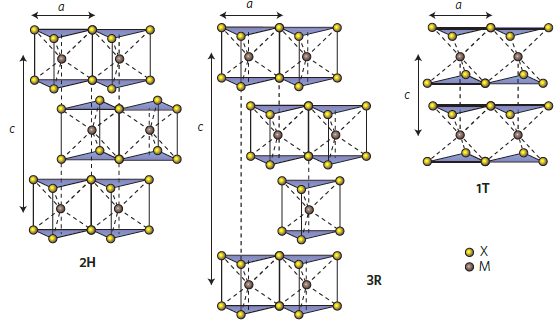
\includegraphics[scale=0.7]{TMDCPolytypes.png}
	\caption{Schematics of the structural polytypes: 2H (hexagonal symmetry, two layers per repeat unit, trigonal prismatic coordination), 3R (rhombohedral symmetry, three layers per repeat unit, trigonal prismatic coordination) and 1T (tetragonal symmetry, one layer per repeat unit, octahedral coordination). The chalcogen atoms (X) are yellow and the metal atoms (M) are grey. The lattice constants a are in the range 3.1 to 3.7 Å for different materials. Adopted from \cite{TMDCReviewNature2012}}
	\label{fig:TMDCPolytypes}
	\end{center}
	\end{figure}
	
	Since graphene have proven to be difficult to work with in the fields of semiconductors due to its lack of natural finite electronic band gap its role as a successor in electronic and opto-electronic devices remains to be seen. However the techniques learned and effects observed during its characterisation were easily transferred to other layered compounds such as TMDCs. In particular the semiconducting, group VI-based TMDCs, containing sulphur and selenium as chalocgen atoms have proven to be more readily potentially useful as an active material in electronic and opto-electronic devices. This is due to their inherent electronic and optical bandgap in visible-near IR range. 
	
	As the number of layers changes from bulk to monolayer the properties of the TMDC undergo a significant change. In most TMDCs the bandgap changes from indirect to a larger direct one. 
	
	\subsection{Electronic properties}
	\label{subsec:Electronic properties}
	
	One of the most interesting features that the layered TMDC materials exhibit is the shift in the bandstructure with the changing number of layers. Several studies have shown in simulations and experimentally that TMDCs have very similar electronic band structure as seen in example of $WS_2$ in Figure \ref{fig:WS2BandStructureSimulation}. In bulk $WS_2$ the maximum of the valence band (VBM) at $\Gamma$ point and the minimum of the conduction band (CBM) at $\Lambda$ form an indirect bandgap. As the number of the layers decreases the CBM at $\Lambda$ point as well as VBM at $K$ point increases causing the band gap to widen. At 2 layers the $K$ point becomes the actual CBM and a new indirect bandgap forms between $\Gamma$ point and $K$ point. Finally in a $WS_2$ monolayer the VBM at $K$ point as well as entire conduction band increases to form a new greater direct band gap at $K$ point. This means that $WS_2$ bandgap changes from 1.3 eV indirect bandgap in bulk to 2.1 eV direct bandgap in monolayer.
	
	\begin{figure}[h]
	\begin{center}
	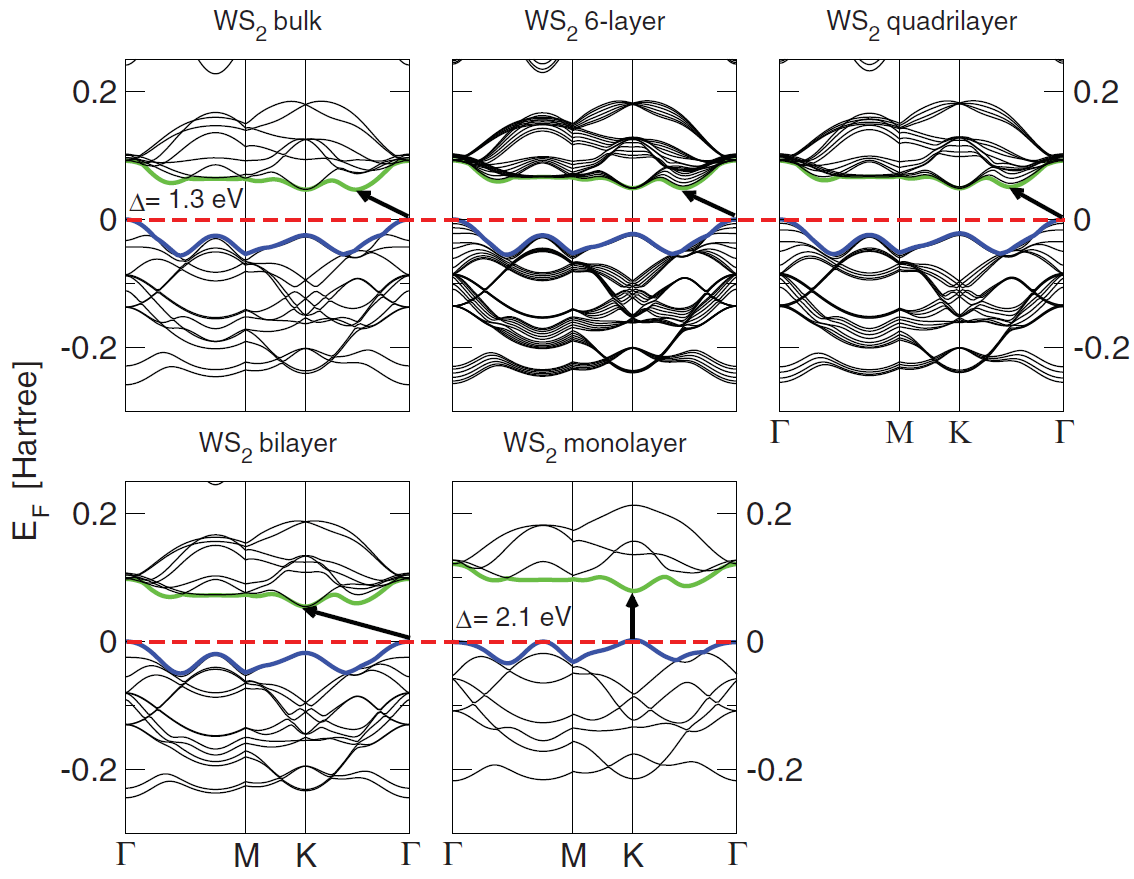
\includegraphics[scale=0.4]{WS2BandStructureSimulation.png}
	\caption{Band structures of bulk $WS_2$, its monolayer, as well as, polylayers calculated from the density functional theory (DFT) simulation. The horizontal dashed lines indicate the Fermi level. The arrows indicate the fundamental band gap (direct or indirect) for a given system. The top of valence band (blue) and bottom of conduction band (green) are highlighted. Adopted from Ref. \cite{WS2BandStructureSimulation}}
	\label{fig:WS2BandStructureSimulation}
	\end{center}
	\end{figure}
	
	 Like $WS_2$ other Mo and W based TMDC undergo similar transitions as seen in Table \ref{tab:MoWBandgapsComparison}. In all cases the smaller indirect bandgap changes to greater direct bandgap with monolayer bandgap ranging from 1.1 eV to about 2.1 eV. Moreover the VBM at K points exhibits the orbit-spin band splitting at the K point of about 400 meV. This direct bandgap leads to presence of A and B excitons generated by transition between CBM and two VBMs at the K point. The conduction band as well as the valence band are dominated by the d-electron orbitals of the transition metal atoms and at the VBM and CBM they hybridize with the p-electron orbitals of the chalcogenide atoms. Because the hybridization happens mostly at the $\Gamma$ point and the chalcogenide atoms are at the surface of the TMDC layer it leads to strong interactions between the layers. This leads to significant change in the band structure at the $\Gamma$ and rise of the indirect bandgap as a result of increased number of layers. On the other hand at the $K$ point the d-orbitals of the transition metals remain mostly unaffected due to them being positioned in the middle of the layer \cite{WS2BandStructureSimulation} \cite{EmergingPhotoluminescenceInMonolayerMoS2}
	 
	 \begin{table}[h]
	 \caption{Mo and W based TMDC bandgaps comparison}
	 \label{tab:MoWBandgapsComparison}
	 \end{table}
	 
	 \begin{center}
	 \begin{tabular}{c|l|l|l}
	 
	 M$\backslash$X & $-S_2$ 			& $-Se_2$ 	& $-Te_2$\\ \hline
	 $Mo$ 			& Semiconducting	& Semiconducting	& Semiconducting	\\ 
	 				& 1L:1.8 eV			& 1L: 1.5 eV		& 1L: 1.1 eV		\\
	 				& Bulk: 1.2 eV		& Bulk: 1.1 eV		& Bulk: 1.0 eV		\\ \hline
	 W 				& Semiconducting	& Semiconducting	& Semiconducting	\\
	 				& 1L:2.1 eV			& 1L: 1.7 eV		& 1L: 1.1 eV		\\
	 				& Bulk: 1.4 eV		& Bulk: 1.2 eV		& 					\\
	 
	 \end{tabular}
	 \end{center}
	
	
	\subsection{Optical properties}
	\label{subsec:Optical properties}

		TMDCs exhibit a wide array of opto-electronic effects due to their strong light-matter effects. These effects are mostly caused by the abundant presence of excitons, bi-excitons, trions or bound excitons. As a result the change in layer thickness from bulk to monolayer alters the photoluminescence, photoconductivity and absorption in the visible to infrared range.
		
		The primary and most common quasi-particle that forms in such system is an exciton, which is a pair of a negatively charged electron and a positively charged hole bound together by Coulomb forces to form a structure similar to that of hydrogen atom. Such pair is electrically neutral and is of size exceeding size of single cell which makes it a Wannier–Mott exciton. The recombination of these excitons results in a photon emission which can be easily observed during photoluminescence characterisation. On top of excitons other quasi-particles such as trions, bi-excitons or bound excitons can be found. A trion is a group of 2 electrons and a hole or 2 holes and an electron, or otherwise described as a charged exciton. The exact nature of the trion depends usually on the type of intrinsic doping of the TMDC. A bi-exciton is a pair of excitons which is usually only observed in quantum dot systems but can be also seen in excitonically dense systems such as TMDCs. A bound exciton is similar to the free exciton but is trapped by a defect. In a typical photoluminescence spectrum several peaks can be observed depending on specific type of TMDC characterised. In $WS_2$ monolayer for instance as seen in Figure. \ref{fig:WS2TypicalPLSpectra} the strongest peak (often labelled as an A peak) at about 1.97 eV is caused by the direct transition of single-photon generated exciton. Slightly redshifted by about 30 meV from the A peak a generally weaker peak caused by the trion recombination can be found. At higher energies another peak can be observed due to the presence of bi-excitons. At around the 1.3 eV a much weaker peak (I) can be seen caused by the indirect transition. Additionally a B peak can be observed blueshifted from the A peak which is caused by valley splitting as discussed in chapter \ref{subsec:Electronic properties}. As seen in Figure \ref{fig:WS2TypicalPLSpectra} as the number of layers increases the main A peak becomes dramatically weaker due to lack of direct transition and redshifted following the pattern discussed in chapter \ref{subsec:Electronic properties}. At the same time the I peak becomes relatively stronger and eventually dominates the bulk material.
		
		\begin{figure}[h]

		\caption{Typical PL spectra of $WS_2$}
		\label{fig:WS2TypicalPLSpectra}
		\end{figure}
		
		Similarly the photoconductivity of the TMDCs is strongly reliant on the number of layers and incident photon energy. The $MoS_2$ for instance shows 3 times stronger photoconductivity in monolayer around 1.8 eV, where the direct transition is located, than in 2L $MoS_@$ around 1.6 eV. Additionally the photoconductivity appears to increase in steps with relation to the photon energy following the direct and indirect transitions. \cite{ElectronicsAndOptoelectronicsOfTwo-dimensionalTransitionMetalDichalcogenides}.
		
		The sunlight absorption in TMDCs has been shown to be significantly more intense than in commonly used solar cell materials, at about 5-10$\%$ which is an order of magnitude greater compared to similar thickness of Si or GaAs. It is also stronger compared to 2-3$\%$ of sunlight absorption of graphene. As a result a excitonic solar cell based on $MoS_2/WS_2$ bilayer shows about 1$\%$ power efficiency, about 3 times greater than that of typical ultrathin solar cells \cite{ExtraordinarySunlightAbsorptionAndOneNanometerThickPhotovoltaicsUsingTwo-DimensionalMonolayerMaterials}.
	
	\subsection{Phonon dispersion}
	\subsection{Heterostructures}
	\subsection{Applications}
\section{Methods}
	\subsection{Raman spectroscopy theory}
	\subsection{Photoluminescence spectroscopy theory}
	\subsection{XPS theory}
\section{Characterisation of $WS_2$}
	\subsection{Optical microscopy of $WS_2$ flakes}
	\subsection{Raman spectroscopy of $WS_2$}
		\subsubsection{Interlayer interactions}
		\subsubsection{Strain}
		\subsubsection{Grain boundaries}
	\subsection{Photoluminescence spectroscopy}
		\subsubsection{PL of $WS_2$ monolayer}
		\subsubsection{PL variation vs flake size}
		\subsubsection{PL variation vs synthesis conditions}
		\subsubsection{Spatial PL variation}
		\subsubsection{Effects of water and oxygen on PL}
\section{Transfer of mono- and fewlayer $WS_2$}
	\subsection{Motivation}
	\subsection{Wet transfer}
		\subsubsection{Methods}
		\subsubsection{Effects on optical and electronic properties}
	\subsection{Dry transfer}
		\subsubsection{Methods}
		\subsubsection{Effects on optical and electronic properties}
\section{Low temperature characterisation of $WS_2$}
	\subsection{Setup}
	\subsection{Isolating trions and excitions}
	\subsection{Spatial variation of PL}
\section{In doped $WS_2$}
	\subsection{Doping theory}
	\subsection{Quantifying In doping}
	\subsection{Effects of doping on PL}
	\subsection{Effects of doping on Raman spectroscopy}
\section{Heterostructures}
	\subsection{Introduction}
	\subsection{Synthesis}
	\subsection{Raman and PL characteristics}
\section{Applications}
	\subsection{Transistors}
	\subsection{LEDs}
	\subsection{Transparent electrodes}
	
\section*{References}
\section*{Appendix}

\section*{Publications}

F. Reale \textit{et al}, "High-Mobility and High-Optical Quality Atomically Thin $WS_2$" Scientific Reports, 2017 - submitted\\ \\
F. M. Pesci \textit{et al}, "MoS2/WS2 heterojunction for photoelectrochemical water oxidation", ACS Catalysis, 2017 - accepted

\section*{Conferences}

Graphene Week, 13-17 June, 2016. (Best poster)\\ \\
UK Semiconductors, 14-15 July, 2017.\\ \\
MRS Boston, 26 November - 1 December, 2017.

\bibliographystyle{plain}
\bibliography{bibliography}{}

\end{document}